%!TEX ROOT=formularioFisica.tex

\section{Gravitazione}\label{sec:gravitazione}
La gravitazione si occupa di studiare le forze che intercorrono tra corpi celesti.\\ 
Essendo le orbite ellittiche (come dice la prima legge di Keplero), $a$ e $b$ si riferiscono ai 
semiassi rispettivamente maggiore e minore.
\begin{center}
	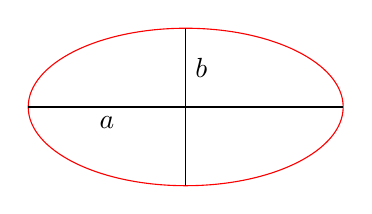
\begin{tikzpicture}	
	\draw[red] ellipse (2 and 1);
	\draw (-2,0) -- ++(4,0)
		node[pos=0.25,below]{$a$};
	\draw (0,1) -- ++(0,-2)
		node[pos=0.25,right]{$b$};
	\end{tikzpicture}
\end{center}
Un pianeta rimane in orbita se la foza di gravita (che attrae verso l'altro corpo/pianeta) ha la 
stessa intensità della forza centrifuga.\\
Per gli esercizi si vada a pagina~\pageref{ex:gravitazione}.

\subsection{Seconda legge di Keplero}
\textit{Il raggio vettore tra la Terra e il Sole spazia aree uguali in tempi uguali.}

\subsection{Terza legge di Keplero}
\begin{equation*}
\frac{a^3}{T^2} = k\,\left(k = \frac{GM}{4\pi^2}\right)
\end{equation*}
$T$: periodo di rivoluzione\\
$a$: lunghezza del semiasse maggiore\\
$M$: massa del pianeta\\
\hyperref[tab:G]{$G$}: $6.67\cdot10^{-11}\,\text{Nm}^2\text{/kg}^2$

\subsection{Legge di Gravitazione Universale}
\begin{equation*}
F = G\frac{m_1m_2}{r^2}
\end{equation*}
\hyperref[tab:g]{$G$}: $6.67\cdot10^{-11}\,\text{Nm}^2\text{/kg}^2$\\
$m$: massa di un pianeta/corpo\\
$r$: distanza tra i corpi

\subsection{Accelerazione Gravitazionale su un pianeta}
\begin{equation*}
g = G\frac{M}{R^2}
\end{equation*}
\hyperref[tab:g]{$G$}: $6.67\cdot10^{-11}\,\text{Nm}^2\text{/kg}^2$\\
$M$: massa del pianeta\\
$R$: raggio del pianeta

\subsection{Velocità di un satellite}
\begin{equation*}
v = \sqrt{\frac{GM}{R}}
\end{equation*}
\hyperref[tab:g]{$G$}: $6.67\cdot10^{-11}\,\text{Nm}^2\text{/kg}^2$\\
$M$: massa del pianeta\\
$R$: $r + h$: raggio del pianeta più distanza dalla superficie

\subsection{Velocità di fuga}
La velocità di fuga è la velocità che un corpo deve avere per poter entrare in orbita del pianeta.
\begin{equation*}
v = \sqrt{\frac{2GM}{R}}
\end{equation*}
\hyperref[tab:g]{$G$}: $6.67\cdot10^{-11}\,\text{Nm}^2\text{/kg}^2$\\
$M$: massa del pianeta\\
$R$: raggio del pianeta\\
